\documentclass[border=8pt]{standalone}
\usepackage[T1]{fontenc}
\usepackage[utf8]{inputenc}
\usepackage{mathptmx}          % Times, para coincidir con el cuerpo del informe
\usepackage{xcolor}
\usepackage{tikz}
\usetikzlibrary{positioning,arrows.meta,calc,fit,backgrounds,decorations.pathreplacing}

% Paleta (coincide con diagramas/arquitectura.pdf)
\definecolor{localFill}{HTML}{E8EEF6}
\definecolor{localDraw}{HTML}{2F5496}
\definecolor{extFill}{HTML}{F0F0F0}
\definecolor{extDraw}{HTML}{7A7A7A}
\definecolor{arrowCol}{HTML}{3A3A3A}

\begin{document}
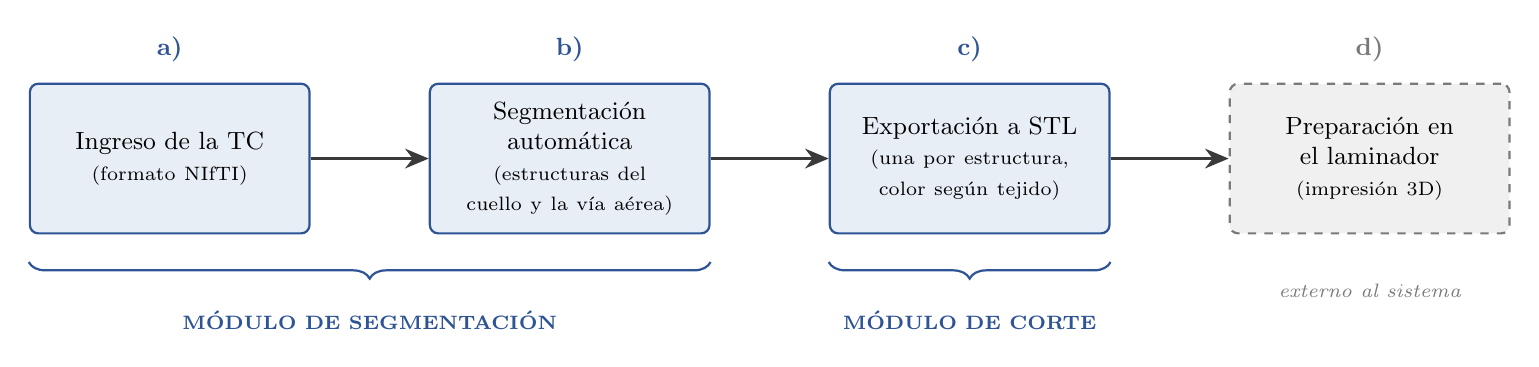
\begin{tikzpicture}[
  font=\small,
  box/.style={draw=localDraw, line width=0.8pt, rounded corners=3pt, fill=localFill,
              align=center, text width=3.2cm, minimum height=1.9cm, inner sep=5pt},
  extbox/.style={draw=extDraw, line width=0.8pt, dashed, rounded corners=3pt, fill=extFill,
              align=center, text width=3.2cm, minimum height=1.9cm, inner sep=5pt},
  flow/.style={-{Stealth[length=3mm,width=2.5mm]}, line width=1.0pt, draw=arrowCol},
  lettr/.style={font=\bfseries\small, text=localDraw, anchor=south},
  lettrext/.style={font=\bfseries\small, text=extDraw, anchor=south},
]

% ---- Las cuatro etapas ----
\node[box]                    (a) at (0,0) {Ingreso de la TC\\\scriptsize(formato NIfTI)};
\node[box, right=1.5cm of a]  (b)          {Segmentación automática\\\scriptsize(estructuras del cuello y la vía aérea)};
\node[box, right=1.5cm of b]  (c)          {Exportación a STL\\\scriptsize(una por estructura, color según tejido)};
\node[extbox, right=1.5cm of c] (d)        {Preparación en el laminador\\\scriptsize(impresión 3D)};

% ---- Etiquetas a) b) c) d) ----
\node[lettr]    at ([yshift=4pt]a.north) {a)};
\node[lettr]    at ([yshift=4pt]b.north) {b)};
\node[lettr]    at ([yshift=4pt]c.north) {c)};
\node[lettrext] at ([yshift=4pt]d.north) {d)};

% ---- Flujo ----
\draw[flow] (a) -- (b);
\draw[flow] (b) -- (c);
\draw[flow] (c) -- (d);

% ---- Brackets de módulos (debajo) ----
\draw[decorate, decoration={brace, amplitude=6pt, mirror}, line width=0.8pt, draw=localDraw]
  ($(a.south west)+(0,-0.35)$) -- ($(b.south east)+(0,-0.35)$);
\node[font=\scriptsize\bfseries, text=localDraw, anchor=north]
  at ($(a.south)!0.5!(b.south)+(0,-0.85)$) {MÓDULO DE SEGMENTACIÓN};

\draw[decorate, decoration={brace, amplitude=6pt, mirror}, line width=0.8pt, draw=localDraw]
  ($(c.south west)+(0,-0.35)$) -- ($(c.south east)+(0,-0.35)$);
\node[font=\scriptsize\bfseries, text=localDraw, anchor=north]
  at ($(c.south)+(0,-0.85)$) {MÓDULO DE CORTE};

\node[font=\scriptsize\itshape, text=extDraw, anchor=north]
  at ($(d.south)+(0,-0.5)$) {externo al sistema};

\end{tikzpicture}
\end{document}